% !TeX spellcheck = en_US
% !TeX encoding = UTF-8
% !TeX root = ../document.tex

\chapter{A Fast Search Algorithm}

In this chapter, the basic concept and method of the Quickscan algorithm is summarized. Arising problems are described and their solutions within the algorithm are proposed. Finally, other approaches are mentioned, which have not been implemented in this work's version of Quickscan.

\section{Concept}
The goal of the Quickscan algorithm is to make the scanning process of pseudo-experiments more efficient. The efficiency improvement is achieved by preselecting interesting regions as RoI (region of interest) candidates and discard most other regions before the costly \p~value calculation.
The selection is performed by evaluating a less computation intensive estimator over all possible connected regions, and making a selection of the most significant deviations according to this estimator. Finally, the full \p~value and its integral are only calculated for the few candidate regions returned by the estimator.

\subsection{The Estimator}
The choice of the estimator plays an important role in the efficiency of the selection. A commonly used quantity in particle physics is 
\begin{equation}
\mychi = \frac{|\Ndata - \Nmc|}{\sigmamc'}
\end{equation}
Here the value $\sigmamc'$ describes the expected deviation. This is not $\sigmamc$ which only includes systematic uncertainties, e.g. finite Monte-Carlo statistics, and has been rescaled to match the data luminosity.
$\sigmamc'$ consists of the expected statistical deviation $\sqrt{\Nmc}$ and the systematical error $\sigmamc$. The two errors are added in quadrature. Because $\Nmc \geq \num{0}$, the expression can be simplified:
\begin{equation}
\sigmamc' \defeq \sqrt{\sigmamc^2 + \left(\sqrt{\Nmc}\right)^2} = \sqrt{\sigmamc^2 + \Nmc}
\end{equation}

This value incorporated into the \mychi-value gives
\begin{equation}
\mychi = \frac{|\Ndata - \Nmc|}{\sqrt{\sigmamc^2 + \Nmc}}
\end{equation}

\subsection{Selection}
In each distribution, the \mychi~value is calculated for each connected bin region. The most significant regions are stored in a list. This introduces a parameter of the Quickscan algorithm, \paramregions, which denotes the \emph{number of candidates} kept in the list.
\begin{figure}
	\centering
	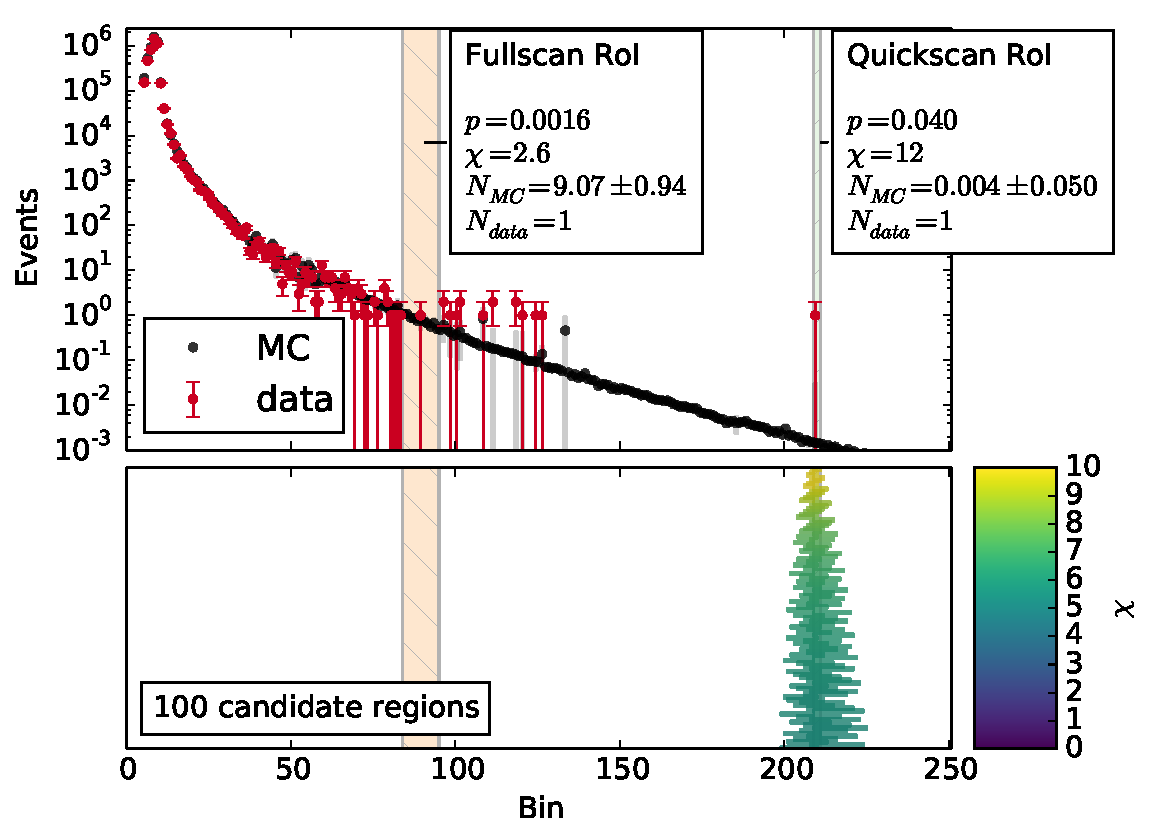
\includegraphics{no_nested_region_handling}
	\caption{Example distribution: Pseudo experiment of the \eventclass{2e} \sumpT distribution, without special treatment of nested regions. The upper panel shows the distribution with the bin number (not the physical quantity) on the horizontal axis and the number of events in each bin on the vertical axis. The lower panel shows the \num{100} selected candidate regions, sorted by \mychi. The regions chosen by the different approaches are indicated in the upper panel. \p denotes the full scan \p~value, while \mychi indicates value of the Quickscan estimator. One can see that especially in the regions where the Poissonian approach $\sigma_N = \sqrt{N}$ fails, the \mychi value is too sensitive. The nested regions suppress different regions in the candidate list, such that the "true" RoI (as found without the Quickscan) is not detected.}
	\label{fig:no_nested_region_handling}
\end{figure}

\subsection{Nested Region Handling}
Using only the estimator and the selection of top \paramregions candidates, the algorithm tends to focus around single data points in the tail of the distribution, where the Poissonian approximation $\sigma_N = \sqrt{N}$ does not hold due to a low event count. This effect is illustrated in figure \ref{fig:no_nested_region_handling}. 
The pseudo experiment of the \eventclass{2e} \sumpT distribution shows a single event above a low background expectation. The regions with the highest \mychi gather around this excess. Comparison with a scan without the new algorithm shows that the "true" region of interest is found further left in the distribution, as a deficit with only \num{1} observed event in \num{9} expected.

To suppress this behavior, an additional list of criteria is introduced, comparing region $A$ with region $B$:
\begin{my_list}
	\item $A$ is nested inside of $B$
	\item Excess of data in $A$: $\Ndata(A) > \Nmc(A)$
	\item Excess of data in $B$: $\Ndata(B) > \Nmc(B)$
	\item No additional data in $B \setminus A$: $\Ndata(A) = \Ndata(B)$
\end{my_list}
If all these conditions are met, then region $A$ is more significant than region $B$.
The mathematical proof for this criterion is difficult, but it can be motivated as follows: If a region contains an excess of observed event yield over MC event yield, and the region is extended while the amount of observed events remains the same, the difference between \Nmc and \Ndata stays equal or is reduced. Since the error \sigmamc can only stay the same or increase, the total significance of the extended region must be less than the original region, as long as it still contains an excess.

\begin{figure}
	\centering
	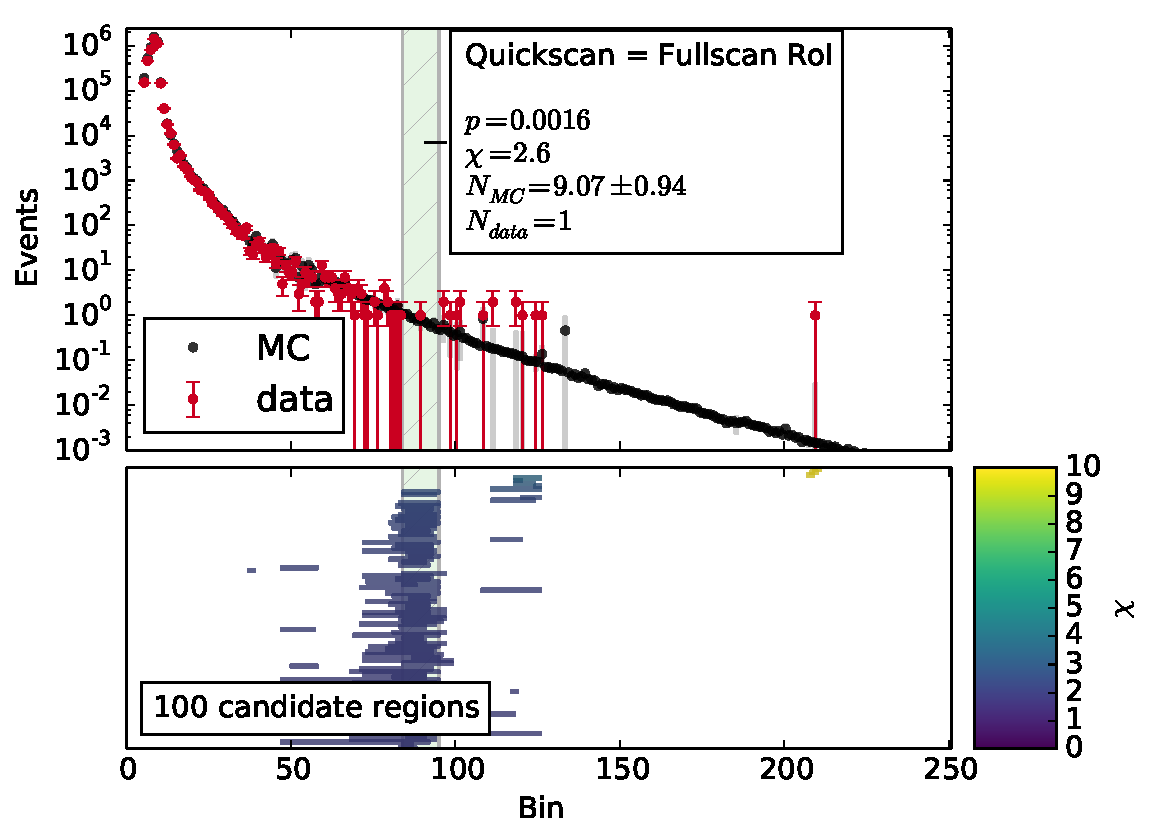
\includegraphics{with_nested_region_handling}
	\caption{Example distribution: pseudo experiment of the \eventclass{2e} \sumpT distribution, with special treatment of nested regions. The scheme is explained below figure \ref{fig:no_nested_region_handling}. This time, only two candidate regions in the high energy tail are selected.}
	\label{fig:with_nested_region_handling}
\end{figure}
Based on this comparison, regions are immediately rejected if a more significant subregion is already included in the candidate list. The results of this treatment can be observed in figure \ref{fig:with_nested_region_handling}. The distribution is exactly the same as in \ref{fig:no_nested_region_handling}, but the algorithm does not focus overly on the event in the tail, leading to the correct RoI to be found.
\FloatBarrier

\section{The Final Algorithm}
The solutions suggested in this chapter are combined in the final algorithm: The Quickscan algorithm maintains a single list of \paramregions candidates for each distribution in each class. Every time a new candidate is considered for insertion into the list, first the nested region criteria are evaluated. If a parent region is found for which the criteria are fulfilled, the candidate immediately replaces the parent region already in the list. Otherwise, its \mychi~value is computed and compared to the candidates in the list. If it is larger than the lowest \mychi inside the list, the region is also inserted.

After all connected regions have been considered, the \p~value is evaluated for the candidate collection and the final region of interest is determined as one of the candidates. 
\newpage 

\section{Running on Pseudo-Experiments Only}
The Quickscan method is only applied to pseudo-experiments, not when calculating the \p~value of measured data, since there might still be cases in which a scan using Quickscan does not find the same region of interest as without. This assures that the data region of interest and its \p~value are definitely correctly computed.

\section{Other Investigated Approaches}
Another method that has been considered during this work is \emph{Magnitude Binning}. This ad-hoc solution also targets the low-statistic regions by individually treating regions with different \Nmc. Instead of keeping one candidate list for an entire distribution, Magnitude Binning keeps one candidate list for each magnitude of \Nmc. The magnitude index is calculated as
\begin{equation}
i = \floor{\log_\parambinbase(\Nmc)} = \floor{\frac{\log(\Nmc)}{\log(\parambinbase)}}
\end{equation}
This introduces a new parameter, \parambinbase, which indicates the size of a magnitude bin. Additionally, the total number of candidate regions is increased by an unknown amount, since the number of orders of magnitude are originally unknown.

This method has been dropped since the other methods proposed in this chapter sufficiently satisfy the Quickscan goals. The Magnitude Binning extension only introduces unnecessary complexity and an additional parameter.

